% ============================================================================
% Barycentre de trois points ponderes
% Extrait de la fiche : Barycentres et lignes de niveau (classe de 1ere D)
% Necessite \usepackage{tikz} et \usetikzlibrary{calc} (charges par le fichier principal)
% ============================================================================
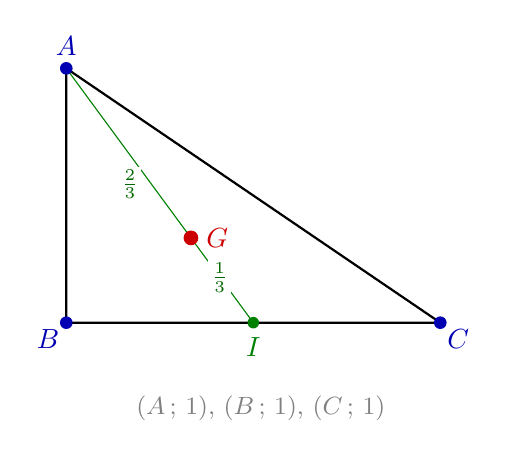
\begin{tikzpicture}[scale=0.95,>=latex]
  \coordinate (A) at (0,3.4); \coordinate (B) at (0,0); \coordinate (C) at (5,0);
  \coordinate (I) at (2.5,0); \coordinate (G) at (1.6667,1.1333);
  \draw[thick] (A) -- (B) -- (C) -- cycle;
  \draw[thin,green!50!black] (A) -- (I);
  \fill[blue!70!black] (A) circle (2.4pt) node[above=1pt] {$A$};
  \fill[blue!70!black] (B) circle (2.4pt) node[below left=-1pt] {$B$};
  \fill[blue!70!black] (C) circle (2.4pt) node[below right=-1pt] {$C$};
  \fill[green!50!black] (I) circle (2.2pt) node[below=2pt] {$I$};
  \fill[red!80!black] (G) circle (2.8pt) node[right=2pt] {$G$};
  \node[green!40!black,font=\small,fill=white,inner sep=1pt] at (0.85,1.85) {$\frac{2}{3}$};
  \node[green!40!black,font=\small,fill=white,inner sep=1pt] at (2.05,0.6) {$\frac{1}{3}$};
  \node[font=\small,gray] at (2.6,-1.15) {$(A\,;\,1)$, $(B\,;\,1)$, $(C\,;\,1)$};
\end{tikzpicture}
